\documentclass{article}
\usepackage{amsmath,amssymb}
\usepackage[margin=3cm]{geometry}
\usepackage{graphicx}
\usepackage{syntax}
\usepackage{dirtree}
\usepackage{longtable}
\usepackage{pgfplots}

\begin{document}

\title{\texttt{randexam}: Randomized Exam Generation and Grading\\[1em] Developer Manual\\[1em] \Large Version 1.13.0}
\date{\vspace*{-2em}2015-10-07}
\maketitle

\section{Concepts}

The exam \emph{library} contains $N_{\rm Q}$ \emph{questions}, each
with up to $N_{\rm V}$ \emph{variants}. Each question variant contains
up to $N_{\rm A}$ \emph{answers}, exactly one of which must be the
\emph{correct answer}. The correct answer for variant $V$ of question
$Q$ is denoted $C(Q,V)$. The questions within the library are grouped
into \emph{zones}.

We randomly generate $N_{\rm e}$ \emph{exams}. Each exam contains
exactly one randomly chosen variant of each library question, with the
question order randomly permuted within each zone. The order of the
zones is not permuted. Questions are numbered globally with the
library and exams, not per-zone. Question $q$ on exam $e$ thus
corresponds to variant $V(e,q)$ of question $Q(e,q)$ in the
library. The answer order for each exam question is also a random
permutation of the original answer order, so $A(e,q,a)$ is the library
answer corresponding to exam answer $a$.

We use capital-letter variables for quantities within the library
and small letters for quantities within the randomly generated exams
and students. Exams, questions, variants, and students are all
numbered with Arabic numerals starting from 1. Answers are numbered
with roman letters starting from A.

Each randomly generated exam is identified by a \emph{key} $K(e)$ of
length $N_{\rm K}$, which is a sequence of answers
$K_1,\ldots,K_{N_K}$. The keys are encoded on the Scantron forms as
the answers to the final set of questions. For example, on a
96-question Scantron form, the 4-digit key ``ECEA'' is encoded as the
answers (93) E, (94) C, (95) E, and (96) A.

During the exam each student completes a single Scantron form,
resulting in $N_{\rm s}$ Scantron forms for an equal number of
students. These forms are scanned and the raw data can be processed to
derive the points for each student.

In summary, the size variables used are:
\begin{center}
  \begin{tabular}{ll}
    $N_{\rm Q}$ & number of questions (in the library and on each exam) \\
    $N_{\rm e}$ & number of exams \\
    $N_{\rm A}$ & maximum number of answers per question \\
    $N_{\rm V}$ & maximum number of variants per question \\
    $N_{\rm s}$ & number of students (equal to the number of Scantron forms) \\
    $N_{\rm g}$ & number of ranked groups of students for statistics generation \\
    $N_{\rm D}$ & number of answer-digits required to encode the exam number \\
    $N_{\rm K}$ & number of answer-digits in the exam key
  \end{tabular}
\end{center}

\section{Processing pipeline}

The full processing pipeline for making, using, and grading a
randomized exam is shown in Figure~\ref{fig:pipeline}. The purple
output files can be inspected and hand-edited before processing runs
to control the processing pipeline.

\begin{figure}
  \centering
  \includegraphics{pipeline}
  \caption{The pipeline for making and grading the randomized
    exams. The green pentagons are input files that require human
    effort to generate, the purple boxes are output files, the yellow
    ellipses are program runs, and the pink hexagon is the students
    sitting the exam and the scanning of the Scantron forms.}
  \label{fig:pipeline}
\end{figure}

\section{File formats}

All library and exam question are formatted in single TeX files. All
data is stored in CSV (comma-separated values) files for easy editing
by hand in a spreadsheet or text editor.

\subsection{\texttt{library.tex}}

The \verb+library_template.tex+ file should be copied to
\verb+library.tex+ and edited to fill in the questions. Non-comment
text may only go into the locations indicated in the file. This file
should be a valid \LaTeX{} file that can be typeset and edited to
prepare the questions. To generate the randomized exams with the
\texttt{randexam} script, the format of \texttt{library.tex} must
conform to the grammar shown in Figure~\ref{fig:library-grammar}. The
basic structure of \texttt{library.tex} is thus a tree, as shown in
Figure~\ref{fig:library-tree}. An outline of the \LaTeX{} in the
\texttt{library.tex} is given in Figure~\ref{fig:library-outline}. The
\texttt{randexam} script processes \texttt{library.tex} using a state
machine. The state transition graph is shown in
Figure~\ref{fig:statemachine}.

\begin{figure}
  \centering
\begin{minipage}{\textwidth}
\setlength{\grammarindent}{9em}
\begin{grammar}
<library> ::= <preamble text> `\verb+\begin{document}+' <body> `\verb+\end{document}+'

<body> ::= <coverpage text> <zone-list>

<zone-list> ::= <zone> <zone-list> | <zone>

<zone> ::= `\verb+\zone+' <zone text>
\alt `\verb+\zone+' <zone text> <question-list>

<question-list> ::= <question> <question-list> | <question>

<question> ::= `\verb+\question{+' <points> `\verb+}+' <variant-list>

<variant-list> ::= <variant> <variant-list> | <variant>

<variant> ::= `\verb+\variant+' <variant text> `\verb+\begin{answers}+' <answer-list> `\verb+\end{answers}+'

<answer-list> ::= <answer> <answer-list> | <answer>

<answer> ::= `\verb+\answer+' <answer text>
\alt `\verb+\correctanswer+' <answer text>
\end{grammar}
\end{minipage}
\caption{Grammer for the \texttt{library.tex} input file expressed in
  partial Backus-Naur Form. The \textit{text} entries refer to any
  valid \LaTeX{} text, and \textit{points} is a numeric value.}
  \label{fig:library-grammar}
\end{figure}

\begin{figure}
  \centering
\begin{minipage}{14em}
\dirtree{%
.1 library.
.2 preamble text.
.2 coverpage text.
.2 zone 1.
.3 zone text.
.3 question 1.
.4 variant 1.
.5 variant text.
.5 answers.
.6 answer 1.
.6 answer 2.
.6 ....
.4 variant 2.
.4 ....
.3 question 2.
.3 ....
.2 zone 2.
.2 ....
}
\end{minipage}
  \caption{Tree structure of the \texttt{library.tex} input file.}
  \label{fig:library-tree}
\end{figure}

\begin{figure}
  \centering
\begin{minipage}{40em}
\begin{verbatim}
<preamble text>
\begin{document}
    <coverpage text>
    \zone
        <zone text>
        \question{<points>}
            \variant
                <variant text>
                \begin{answers}
                    \answer <answer text>
                    \correctanswer <answer text>
                    <more answers...>
                \end{answers}
            <more variants...>
        <more questions...>
    <more zones...>
\end{document}
\end{verbatim}
\end{minipage}
\caption{Outline of the \texttt{library.tex} input file.}
  \label{fig:library-outline}
\end{figure}

\begin{figure}
  \centering
  \includegraphics{statemachine}
  \caption{The state machine used by the \texttt{randexam} script to
    read the \texttt{library.tex} input file.}
  \label{fig:statemachine}
\end{figure}

\subsection{\texttt{exams.tex}}

This is the generated file containing all of the randomized
exams. Each coverpage ends with the exam key that needs to be filled
in by the student.

\subsection{\texttt{specs.csv}}

This file encodes the arrays:
\begin{center}
  \begin{tabular}{lll}
    array & dimensions & description \\
    \hline
    $K(e)$ & $N_{\rm e}$ & key for exam $e$ \\
    $Q(e,q)$ & $N_{\rm e} \times N_{\rm Q}$
    & library question for question $q$ on exam $e$ \\
    $V(e,q)$ & $N_{\rm e} \times N_{\rm Q}$
    & library question variant for question $q$ on exam $e$ \\
    $A(e,q,a)$ & $N_{\rm e} \times N_{\rm Q} \times N_{\rm A}$
    & library answer corresponding to answer $a$ for question $q$ on exam $e$
  \end{tabular}
\end{center}
The first column is the exam number, the second column is the exam
key, and then triples of columns identify the library question $Q$,
variant $V$, and library answer order. As an example:
\begin{verbatim}
e,K(e),"Q(e,q=1)","V(e,q=1)","A(e,q=1,:)","Q(e,q=2)","V(e,q=2)","A(e,q=2,:)"
1,ADC,2,2,DEBCA,3,2,DCEBA
2,BED,1,2,BDCAE,2,1,DECBA
\end{verbatim}
Here the key of the first exam is $K(1) = {\rm ADC}$ and the second
question on this exam is variant $V(1,2) = 2$ of library question
$Q(1,2) = 3$. The first answer for this question on the exam paper is
answer $A(1,2,1) = \rm D$ from the library question, while the second
answer on the exam paper is answer $A(1,2,2) = \rm C$ from the library
question.

\subsection{\texttt{points.csv}}

The points file encodes the array:
\begin{center}
  \begin{tabular}{lll}
    array & dimensions & description \\
    \hline
    $P(Q,V,A)$ & $N_{\rm Q} \times N_{\rm V} \times N_{\rm A}$
    & points awarded for giving answer $A$ to variant $V$ of question $Q$
  \end{tabular}
\end{center}
This is stored as a four-column file with entries like:
\begin{verbatim}
Q,V,A,"P(Q,V,A)"
...
2,1,A,0.0
2,1,B,0.0
2,1,C,0.0
2,1,D,1.0
2,1,E,0.0
\end{verbatim}
Here some lines have been removed, as indicated by the ellipsis. This
shows that for variant 1 of question 2, answer D is worth 1
point and all other answers are not worth any points, so
$P(2,1,4) = 1.0$ and $P(2,1,A) = 0$ for $A \ne 4$.

\subsection{\texttt{override.csv}}

The override file encodes the array:
\begin{center}
  \begin{tabular}{llp{10.5cm}}
    array & dimensions & description \\
    \hline
    $P^{\rm over}_{\rm sQ}$ & $N_{\rm s} \times N_{\rm Q}$
    & override points awarded to student $s$ for library question $Q$
    (or -1 to not override)
  \end{tabular}
\end{center}
This is stored as a CSV file with the first column being the student
NetID and subsequent columns specifying questions. The column header
indicates the question number. It is not necessary to include all
students or all questions, and any students or questions not specified
will have entries of $-1$ in $P^{\rm over}_{\rm sQ}$, indicating that
they should not be overridden. For example:
\begin{verbatim}
NetID,8,13
RDEVILLE,0.4,7
MWEST,0,-1
\end{verbatim}
Here two students have override scores specified for two
questions. Student \texttt{RDEVILLE} will have a score of 0.4 for
library question $Q = 8$ and $7$ for $Q = 13$. Student \texttt{MWEST}
will have a score of zero for question $Q = 8$, but for question $Q =
13$ his score will not be overridden, meaning it will be computed from
the answer and points data as usual.

\subsection{\texttt{solutions.csv}}

This file gives the correct solutions for each exam in case grading by
hand is necessary. This thus encodes the array:
\begin{center}
  \begin{tabular}{lll}
    array & dimensions & description \\
    \hline
    $c(e,q)$ & $N_{\rm e} \times N_{\rm Q}$
    & the correct answer for question $q$ on exam $e$
  \end{tabular}
\end{center}
The first two columns give the exam number and key for reference, and
then subsequent columns give the correct answers. For example:
\begin{verbatim}
e,K(e),"C(e,q=1)","C(e,q=2)","C(e,q=3)"
1,ADC,A,A,D
2,BED,D,A,A
3,CAE,A,E,D
4,DBA,A,A,D
5,ECB,B,E,A
\end{verbatim}
Here the third exam has key $K(3) = \rm CAE$ and the correct answer
for the first question on this exam is $c(3,1) = \rm A$, while the
correct answer for the second question is $c(3,2) = E$, etc.

The correct answers for each exam are derived from the correct answers
in the library file, given for each library question and each variant
in the array:
\begin{center}
  \begin{tabular}{lll}
    array & dimensions & description \\
    \hline
    $C(Q,V)$ & $N_{\rm Q} \times N_{\rm V}$
    & the correct answer for variant $V$ of library question $Q$
  \end{tabular}
\end{center}
The derivation of $c(e,q)$ is then:
\begin{equation}
  A(e,q,c(e,q)) = C\big( Q(e,q), V(e,q) \big).
\end{equation}

\subsection{\texttt{scantron.dat}}

This is the raw data file from the Scantron machine. There are two
possible formats for the Scantron data, depending on whether students
are allowed to bubble in more than one answer. Selecting multiple
answers is a possible approach for partial credit (where a student may
get half or third credit if they select two or three answers, for
example). The difference in the data file is how the answers are
encoded. If only a single answer is allowed, then it contains lines
like:
\begin{verbatim}
721000001001120412001Y  5380     1    N DEVILLE   R993502067   RDEVILLE 434
721000002001120412001Y  5380     1    N WEST      M795969582   MWEST    252
\end{verbatim}
Here each answer is represented by a single digit, with 1 = A, 2 = B,
etc., so student \verb+RDEVILLE+ answered D for question 1, C for
question 2, and D for question 3.

If, instead, multiple answers are allowed, the question information is
encoded in a two-digit decimal value that represents a little-endian
``binary'' encoding of the bubbled answers. That is, each answer has a
numeric value ($2^0$ = A, $2^1$ = B, \ldots, $2^4$ = E) and the
question value is the sum of all selected answer values. The data file
then contains lines like:
\begin{verbatim}
721000001001120412001Y  5380     1    N DEVILLE   R993502067   RDEVILLE 080412
721000002001120412001Y  5380     1    N WEST      M795969582   MWEST    021601
\end{verbatim}
Here student \verb+RDEVILLE+ answered D for question 1 (08 = $2^3$ =
D), C for question 2 (04 = $2^2$ = C), and both C and D for question 3
(12 = $2^2 + 2^3$ = C + D).

The actual file sent from the scanning office should be renamed to
\verb+scantron.dat+. The particular parsing is controlled by the
variable \verb+MULTIPLE_ANSWERS_PER_QUESTION+; this variable only
controls the parsing of \verb+scantron.dat+.

\subsection{\texttt{answers.csv}}

This file is essentially just a CSV version of the data in
\verb+scantron.dat+. It encodes the arrays:
\begin{center}
  \begin{tabular}{lll}
    array & dimensions & description \\
    \hline
    $u(s,i)$ & $N_{\rm s} \times 4$
    & student last name, first initial, student ID number, and NetID \\
    $b(s,q,a)$ & $N_{\rm s} \times N_{\rm Q} \times N_{\rm A}$
    & bubble selection of answer $a$ given to question $q$ by student $s$;\\
    & & 0 = empty, 1 = filled \\
    $k(s)$ & $N_{\rm s}$
    & key filled in by student $s$
  \end{tabular}
\end{center}
The first column in the data file is the student number, then the next
four columns store the student information, the sixth column stores
the exam key, and then columns 7 and up store the bubbled-in answers
to the questions in exam order. As an example:
\begin{verbatim}
s,Name,Initial,Number,NetID,k(s),"b(s,q=1,:)","b(s,q=2,:)","b(s,q=3,:)"
1,DEVILLE,R,993502067,RDEVILLE,CAE,D,C,CD
2,WEST,M,795969582,MWEST,ECB,B,E,AB
\end{verbatim}
Here we see the second student has information giving the last name
$u(2,1) = \mathtt{WEST}$, the first initial $u(2,2) = \mathtt{M}$, the
student number $u(2,3) = 795969582$, and the NetID $u(2,4) =
\texttt{MWEST}$. The exam key for this student is $k(2) = \rm ECB$ and
the student bubbled answers $b(2,1,:) = [0,1,0,0,0]$ (selecting just
B) for question 1 on this exam paper, bubbled answers $b(2,2,:) =
[0,0,0,0,1]$ (selecting just E) for question 2, and bubbled answers
$b(2,3,:) = [1,1,0,0,0]$ (selecting both A and B) for question 3.

\subsection{\texttt{scores.csv}}

This file encodes the array $P_{\rm se}(s)$ described in
Section~\ref{sec:grading}. For reference, the student number and
information in array $u(s,i)$ is also included in the first
columns. As an example:
\begin{verbatim}
s,Name,Initial,Number,NetID,P_s(s)
1,DEVILLE,R,993502067,RDEVILLE,2.0
2,WEST,M,795969582,MWEST,2.0
\end{verbatim}
Here we see that both students have total points $P_{\rm s}(1) =
P_{\rm s}(2) = 2.0$.

\subsection{\texttt{stats.tex}}

This file presents various summary statistics relating to the student
and question performance in the exam. It should be processed with
\texttt{pdflatex} to produce the output \texttt{stats.pdf} file.

\subsection{\texttt{stats\underline{ }*.csv}}

Multiple files are written to encode the statistics arrays described
in Section~\ref{sec:statistics}. These are named after the variables
they contain, so $n^{\rm a}_{\rm QV}$ is be stored in
\verb+stats_n_a_QV.csv+, for example. The format is broadly similar to
those files described in detail above, with column headings that
specify the contents.

\section{Grading}
\label{sec:grading}

The map from student number $s$ to exam number $e$ is given by the
array
\begin{center}
  \begin{tabular}{lll}
    array & dimensions & description \\
    \hline
    $e(s)$ & $N_{\rm s}$ & exam number corresponding to student number $s$
  \end{tabular}
\end{center}
This array is determined so that
\begin{equation}
  K(e(s)) = k(s).
\end{equation}

The points awarded to each student can be determined using the grading
key for any exam, not just the particular exam that the student
actually took. To make this clear, we consider the arrays:
\begin{center}
  \begin{tabular}{lll}
    array & dimensions & description \\
    \hline
    $P_{\rm seq}(s,e,q)$ & $N_{\rm s} \times N_{\rm e} \times N_{\rm Q}$
    & points awarded to student $s$ on question $q$ scored for exam $e$ \\
    $P_{\rm se}(s,e)$ & $N_{\rm s} \times N_{\rm e}$
    & total points awarded to student $s$ scored for exam $e$ \\
    $P_{\rm sq}(s,q)$ & $N_{\rm s} \times N_{\rm Q}$
    & points award to student $s$ on question $q$ using the correct exam \\
    $P_{\rm s}(s)$ & $N_{\rm s}$
    & total points awarded to student $s$ scored using the correct exam \\
    $P_{\rm sQ}(s,Q)$ & $N_{\rm s} \times N_{\rm Q}$
    & points awarded to student $s$ for library question $Q$
  \end{tabular}
\end{center}
We define an array for partial credit $\sigma(n)$ (the variable
\verb+SCORE_PER_ANSWERS+ in \verb+randexam+) which is the score value
multiplier when $n$ answers are selected (e.g., $\sigma(1)=1$ always,
but $\sigma(n)=1/n$ can be used to award partial credit, or
$\sigma(n)=0$ for $n>1$ will allow no partial credit). The first array
in the table above is computed by:
\begin{equation}
  P_{\rm seq}(s,e,q) = \begin{cases}
    \displaystyle \sum_{a=1}^{N_{\rm A}} P\Big(Q(e,q), V(e,q), A(e,q,a)\Big)
    b(s,q,a) \sigma\Bigg(\sum_{a'=1}^{N_{\rm A}} b(s,q,a')\Bigg)
    & \text{if } P^{\rm over}_{\rm sQ}\big(s,Q(e,q)\big) < 0 \\
    P^{\rm over}_{\rm sQ}\big(s,Q(e,q)\big) & \text{otherwise}
  \end{cases}
\end{equation}
The subsequent arrays in the table above are then computed by:
\begin{align}
  P_{\rm se}(s,e) &= \sum_{q = 1}^{N_{\rm Q}} P_{\rm seq}(s,e,q) \displaybreak[0] \\
  P_{\rm sq}(s,q) &= P_{\rm seq}\big(s,e(s),q\big) \displaybreak[0] \\
  P_{\rm s}(s) &= P_{\rm se}\big(s,e(s)\big) \displaybreak[0] \\
  P_{\rm sQ}\Big(s,Q\big(e(s),q\big)\Big) &= P_{\rm seq}\big(s,e(s),q\big).
\end{align}
We expect that $e(s)$ maximizes $P_{\rm se}(s,e)$ for each $s$, as
grading with the ``wrong'' exam key should give random choices for
each answer. Indeed, for $\hat{e} \ne e(s)$, $P_{\rm se}(s,\hat{e})$
should be approximately $N_{\rm Q} / N_{\rm A}$, assuming that each
question is worth one point if correct. Some significant deviations
are likely, however, when the number of students $N_{\rm s}$ is much
larger than the number of questions $N_{\rm Q}$.

\section{Curving}
\label{sec:curving}

Curved score values are stored in the array:
\begin{center}
  \begin{tabular}{lll}
    array & dimensions & description \\
    \hline
    $P^{\rm curve}_{\rm s}(s)$ & $N_{\rm s}$
    & total curved points awarded to student $s$
  \end{tabular}
\end{center}

The default is for no curving, in which case $P^{\rm curve}_{\rm s}$
is equal to $P_{\rm s}$. If score curving is enabled (by the
\texttt{curve_scores} configuration parameter) then
$P^{\rm curve}_{\rm s}$ is computed using the piecewise linear
function shown in Figure~\ref{fig:curve} with the following
parameters:
\begin{center}
  \begin{tabular}{cll}
    quantity & config option & description \\
    \hline
    $M_0$ & --- & median of old (uncurved) scores \\
    $M_1$ & \texttt{curve_new_median} & desired median of new (curved) scores \\
    $Z_1$ & \texttt{curve_new_zero} & desired new (curved) score for old zero score
  \end{tabular}
\end{center}

\begin{figure}
  \centering
  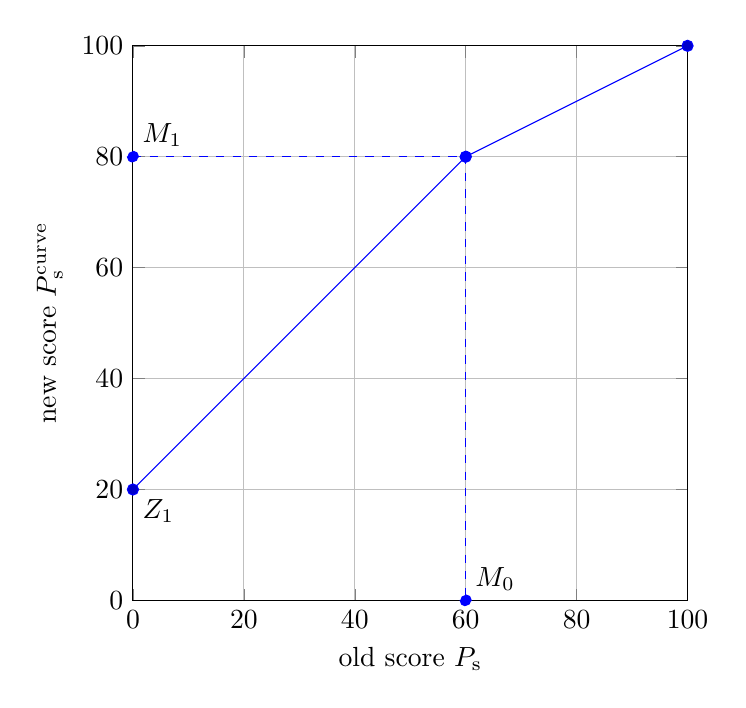
\begin{tikzpicture}
    \begin{axis}[
      width=10cm,
      xlabel={old score $P_{\rm s}$},
      ylabel={new score $P^{\rm curve}_{\rm s}$},
      grid=both,
      axis equal image,
      xmin=0,
      xmax=100,
      ymin=0,
      ymax=100,
      ]
      \node[above right] at (axis cs:60,0) {$M_0$};
      \node[above right] at (axis cs:0,80) {$M_1$};
      \node[below right] at (axis cs:0,20) {$Z_1$};
      \addplot coordinates {
        (0,20)
        (60,80)
        (100,100)
      };
      \addplot[dashed,blue,mark=*] coordinates {
        (0,80)
        (60,80)
        (60,0)
      };
    \end{axis}
  \end{tikzpicture}
  \caption{Curving function that transforms old scores to new scores.}
  \label{fig:curve}
\end{figure}

\section{Statistics}
\label{sec:statistics}

As well as computing the scores for each student, we can assess how
the students as a group performed on the different questions and
variants. Basic statistics for this assessment are listed below.
  \begin{longtable}[c]{llp{9cm}}
    array & dimensions & description \\
    \hline
    \endhead
    $n^{\rm s}_{\rm e}(e)$ & $N_{\rm e}$
    & number of students taking exam $e$ \\
    $n^{\rm s}_{\rm QV}(Q,V)$ & $N_{\rm Q} \times N_{\rm V}$
    & number of students given variant $V$ of question $Q$ \\
    $n^{\rm a}_{\rm QVA}(Q,V,A)$ & $N_{\rm Q} \times N_{\rm V} \times N_{\rm A}$
    & number of students giving answer $A$ for variant $V$ of question $Q$ \\
    $n^{\rm a}_{\rm QV}(Q,V)$ & $N_{\rm Q} \times N_{\rm V}$
    & number of students giving an answer for variant $V$ of question $Q$ \\
    $n^{\rm na}_{\rm QV}(Q,V)$ & $N_{\rm Q} \times N_{\rm V}$
    & number of students not giving an answer for variant $V$ of question $Q$ \\
    $n^{\rm a}_{\rm Q}(Q)$ & $N_{\rm Q}$
    & number of students giving an answer for question $Q$ \\
    $r^{\rm a}_{\rm QVA}(Q,V,A)$ & $N_{\rm Q} \times N_{\rm V} \times N_{\rm A}$
    & fraction of students giving answer $A$ for variant $V$ of question $Q$ \\
    $r^{\rm na}_{\rm QV}(Q,V)$ & $N_{\rm Q} \times N_{\rm V}$
    & fraction of students not giving an answer for variant $V$ of question $Q$ \\
    $P_{\rm QV}(Q,V)$ & $N_{\rm Q} \times N_{\rm V}$
    & total points awarded for variant $V$ of question $Q$ \\
    $P_{\rm Q}(Q)$ & $N_{\rm Q}$
    & total points awarded for question $Q$ \\
    $\bar{P}_{\rm QV}(Q,V)$ & $N_{\rm Q} \times N_{\rm V}$
    & average points per student for variant $V$ of question $Q$ \\
    $\bar{P}_{\rm Q}(Q)$ & $N_{\rm Q}$
    & average points per student for question $Q$ \\
    $\bar{P}$ & 1
    & average points per student for entire exam \\
    $P^{\rm max}_{\rm QV}(QV)$ & $N_{\rm Q} \times N_{\rm V}$
    & maximum points available for variant $V$ of question $Q$ \\
    $P^{\rm max}_{\rm Q}(Q)$ & $N_{\rm Q}$
    & maximum points available for question $Q$ \\
    $P^{\rm max}$ & $1$
    & maximum points available for the entire exam \\
    $\hat{P}_{\rm Q}(Q)$ & $N_{\rm Q}$
    & normalized average points per student for question $Q$ \\
    $R_{\rm QV}(Q,V)$ & $N_{\rm Q} \times N_{\rm V}$
    & ratio of average points for variant $V$ to average for question $Q$ \\
    $n_{\rm QVC}(Q,V,C)$ & $N_{\rm Q} \times N_{\rm V} \times N_{\rm A}$
    & number of students who bubbled in $C$ answers for variant $V$ of question $Q$ \\
    $r^{\rm s}_{QQ}(Q,\hat{Q})$ & $N_{\rm Q} \times N_{\rm Q}$
    & correlation between student scores on questions $Q$ and $\hat{Q}$ \\
    $r^{\rm Q}_{\rm ss}(s,\hat{s})$ & $N_{\rm s} \times N_{\rm s}$
    & correlation between question points for students $s$ and $\hat{s}$ \\
    $n^{\rm ai}_{\rm ss}(s,\hat{s})$ & $N_{\rm s} \times N_{\rm s}$
    & number of mutually incorrect exam answers for students $s$ and $\hat{s}$ \\
    $r^{\rm ai}_{\rm ss}(s,\hat{s})$ & $N_{\rm s} \times N_{\rm s}$
    & proportion of identical incorrect answers for students $s$ and $\hat{s}$ \\
    $D_{\rm Q}(Q)$ & $N_{\rm Q}$
    & ``difficulty'' of question $Q$: one minus normalized averaged points $\hat{P}_{\rm Q}(Q)$ \\
    $r^{\rm P}_{\rm Q}(Q)$ & $N_{\rm Q}$
    & ``discrimination'' of question $Q$: correlation coefficient of $P_{\rm sQ}(s,Q)$ and $\big(P_{\rm s}(s) - P_{\rm sQ}(s,Q)\big)$ \\
    $q_{\rm sQ}(s,Q)$ & $N_{\rm s} \times N_{\rm Q}$
    & exam question number $q$ in which library question $Q$ appears for student $s$ \\
    $V_{\rm sQ}(s,Q)$ & $N_{\rm s} \times N_{\rm Q}$
    & variant number of library question $Q$ given to student $s$ \\
    $c_{\rm sQ}(s,Q)$ & $N_{\rm s} \times N_{\rm Q}$
    & correct answer position for library question $Q$ given to student $s$
  \end{longtable}
These quantities are computed by:
\begin{align}
  n^{\rm s}_{\rm e}(e) &= \sum_{s = 1}^{N_{\rm s}} \delta\big(K(e), k(s)\big) \displaybreak[0] \\
  n^{\rm s}_{\rm QV}(\hat{Q},\hat{V}) &= \sum_{s = 1}^{N_{\rm s}} \sum_{q = 1}^{\rm N_{\rm Q}}
  \delta\Big(\hat{Q}, Q\big(e(s),q\big)\Big)
  \ \delta\Big(\hat{V}, V\big(e(s),q\big)\Big) \displaybreak[0] \\
  n^{\rm a}_{\rm QVA}(\hat{Q},\hat{V},\hat{A}) &= \sum_{s = 1}^{N_{\rm s}} \sum_{q = 1}^{N_{\rm Q}} \sum_{a = 1}^{N_{\rm A}}
  \delta\Big( \hat{Q}, Q\big(e(s),q\big) \Big) \ \delta\Big(\hat{V}, V\big(e(s),q\big) \Big)
  \ \delta\Big( \hat{A}, A\big(e(s),q,a\big) \Big) \nonumber \\
  &\qquad \cdot b(s,q,a)\sigma\Big(\sum_{a'}b(s,q,a')\Big) \displaybreak[0] \\
  n^{\rm a}_{\rm QV}(Q,V) &= \sum_{A = 1}^{N_{\rm A}} n^{\rm a}_{\rm QVA}(Q,V,A) \displaybreak[0] \\
  n^{\rm na}_{\rm QV}(Q,V) &= n^{\rm s}_{\rm QV}(Q,V) - n^{\rm a}_{\rm QV}(Q,V) \displaybreak[0] \\
  n^{\rm a}_{\rm Q}(Q) &= \sum_{V = 1}^{N_{\rm V}} n^{\rm a}_{\rm QV}(Q,V) \displaybreak[0] \\
  r^{\rm a}_{\rm QVA}(Q,V,A) &= \frac{n^{\rm a}_{\rm QVA}(Q,V,A)}{n^{\rm s}_{\rm QV}(Q,V)} \displaybreak[0] \\
  r^{\rm na}_{\rm QV}(Q,V) &= \frac{n^{\rm na}_{\rm QV}(Q,V)}{n^{\rm s}_{\rm QV}(Q,V)} \displaybreak[0] \\
  P_{\rm QV}(\hat{Q},\hat{V}) &= \sum_{s = 1}^{N_{\rm s}} \sum_{q = 1}^{N_{\rm Q}} P_{\rm sq}(s,q)
  \ \delta\Big(\hat{Q}, Q\big(e(s),q\big)\Big)
  \ \delta\Big(\hat{V}, V\big(e(s),q\big)\Big) \displaybreak[0] \\
  P_{\rm Q}(Q) &= \sum_{V = 1}^{N_{\rm V}} P_{\rm QV}(Q,V) \displaybreak[0] \\
  \bar{P}_{\rm QV}(Q,V) &= \frac{P_{\rm QV}(Q,V)}{n^{\rm s}_{\rm QV}(Q,V)} \displaybreak[0] \\
  \bar{P}_{\rm Q}(Q) &= \frac{P_{\rm Q}(Q)}{N_{\rm s}} \displaybreak[0] \\
  \bar{P} &= \sum_{Q=1}^{N_{\rm Q}} \bar{P}_{\rm Q}(Q)
  = \frac{1}{N_{\rm s}} \sum_{s=1}^{N_{\rm s}} P_{\rm s}(s) \displaybreak[0] \\
  P^{\rm max}_{\rm QV}(Q,V) &= \max_{A \in \{1,\ldots,N_{\rm A}\}} P(Q,V,A) \displaybreak[0] \\
  P^{\rm max}_{\rm Q}(Q) &= \max_{V \in \{1,\ldots,N_{\rm V}\}} P^{\rm max}_{\rm QV}(Q,V) \displaybreak[0] \\
  P^{\rm max} &= \sum_{Q=1}^{N_{\rm Q}} P^{\rm max}_{\rm Q}(Q) \displaybreak[0] \\
  \hat{P}_{\rm Q}(Q) &= \frac{\bar{P}_{\rm Q}(Q)}{P^{\rm max}_{Q}(Q)} \displaybreak[0] \\
  R_{\rm QV}(Q,V) &= \frac{\bar{P}_{\rm QV}(Q,V)}{\bar{P}_{\rm Q}(Q)} \displaybreak[0] \\
  n_{\rm QVC}(Q,V,C) &= \sum_{s=1}^{N_{\rm s}} \delta\left(C - \sum_{a=1}^{N_{\rm A}} b\big(s,q_{\rm sQ}(s,Q),a\big)\right)
  \delta\big(V-V_{\rm sQ}(s,Q)\big) \displaybreak[0]\\
  r^{\rm s}_{\rm QQ}(Q, \hat{Q}) &= \frac{\sum_{s=1}^{N_{\rm s}}
    (P_{sQ}(s,Q) - \bar{P}_Q(Q)) (P_{sQ}(s,\hat{Q}) - \bar{P}_Q(\hat{Q}))
  }{
    \sqrt{\sum_{s=1}^{N_{\rm s}} (P_{sQ}(s,Q) - \bar{P}_Q(Q))^2}
    \sqrt{\sum_{s=1}^{N_{\rm s}} (P_{sQ}(s,\hat{Q}) - \bar{P}_Q(\hat{Q}))^2}} \displaybreak[0] \\
  r^{\rm Q}_{\rm s}(s, \hat{s}) &= \frac{\sum_{Q=1}^{N_{\rm Q}}
    (P_{sQ}(s,Q) - \bar{P}_Q(Q)) (P_{sQ}(s,\hat{Q}) - \bar{P}_Q(\hat{Q}))
  }{
    \sqrt{\sum_{Q=1}^{N_{\rm Q}} (P_{sQ}(s,Q) - \bar{P}_Q(Q))^2}
    \sqrt{\sum_{Q=1}^{N_{\rm Q}} (P_{sQ}(s,\hat{Q}) - \bar{P}_Q(\hat{Q}))^2}} \displaybreak[0] \\
  n^{\rm ai}_{\rm ss}(s,\hat{s}) &= \sum_{q = 1}^{N_{\rm Q}} \delta\big(0, P_{\rm sq}(s,q)\big)
  \ \delta\big(0, P_{\rm sq}(\hat{s},q)\big) \displaybreak[0] \\
  r^{\rm ai}_{\rm ss}(s,\hat{s}) &= \frac{1}{n^{\rm ai}_{\rm ss}(s,\hat{s})} \sum_{q = 1}^{N_{\rm Q}}
  \delta\big(a(s,q), a(\hat{s},q)\big)
  \ \delta\big(0, P_{\rm sq}(s,q)\big) \ \delta\big(0, P_{\rm sq}(\hat{s},q)\big) \displaybreak[0] \\
  D_{\rm Q}(Q) &= 1 - \hat{P}_{\rm Q}(Q) \displaybreak[0] \\
  r^{\rm P}_{\rm Q}(Q) &= \frac{\displaystyle \sum_{s=1}^{N_{\rm s}}
    \Big(P_{sQ}(s,Q) - \bar{P}_Q(Q)\Big) \Big(\big(P_{s}(s) - P_{sQ}(s,Q)\big) - \big(\bar{P} - \bar{P}_Q(Q)\big)\Big)
  }{
    \sqrt{\displaystyle \sum_{s=1}^{N_{\rm s}} \Big(P_{sQ}(s,Q) - \bar{P}_Q(Q)\Big)^2}
    \sqrt{\displaystyle \sum_{s=1}^{N_{\rm s}} \Big(\big(P_{s}(s) - P_{sQ}(s,Q)\big) - \big(\bar{P} - \bar{P}_Q(Q)\big)\Big)^2}} \displaybreak[0] \\
  q_{\rm sQ}(s,\hat{Q}) &= \sum_{q = 1}^{N_{\rm Q}} \delta\Big(\hat{Q},Q\big(e(s),q\big)\Big) q
  \hspace{2em} \Longrightarrow \hspace{2em} Q\big(e(s), q_{\rm sQ}(s,\hat{Q})\big) = \hat{Q} \displaybreak[0] \\
  V_{\rm sQ}(s,Q) &= V\big(e(s), q_{\rm sQ}(s,Q)\big) \\
  c_{\rm sQ}(s,Q) &= c\big(e(s), q_{\rm sQ}(s,Q)\big)
\end{align}
where $\delta(x,y)$ is the Kronecker delta function, equal to one with
equal arguments and zero otherwise.

We expect that $R_{\rm QV}(Q,V) \approx 1$, indicating that all
variants were equally difficult for question $Q$. We also expect that
$r^{\rm ai}_{\rm ss}(s,\hat{s}) \approx 1/N_{\rm A}$ for $e(s) =
e(\hat{s})$, indicating only random association between incorrect
answers given by students with identical exams, although this may be
legitimately higher due to correlations between student mistakes.

To understand how students of different ability levels perform it is
helpful to group students by their exam scores. We consider $N_{\rm
  g}$ almost-equal-sized \emph{groups} of students, where all students
in group $g$ perform worse than all students in group $g + 1$, etc. We
can then compute the following per-group quantities:
\begin{center}
  \begin{tabular}{llp{9cm}}
    array & dimensions & description \\
    \hline
    $s(r)$ & $N_{\rm s}$
    & student number at rank $r$ \\
    $g(s)$ & $N_{\rm g}$
    & group number of student $s$ \\
    $n^{\rm s}_{\rm g}(g)$ & $N_{\rm g}$
    & number of students in group $g$ \\
    $P_{\rm gQV}(g,Q,V)$ & $N_{\rm g} \times N_{\rm Q} \times N_{\rm V}$
    & total points awarded for variant $V$ of question $Q$ to students in group $g$ \\
    $P_{\rm gQ}(g,Q)$ & $N_{\rm g} \times N_{\rm Q}$
    & total points awarded for question $Q$ to students in group $g$ \\
    $\bar{P}_{\rm gQ}(g,Q)$ & $N_{\rm g} \times N_{\rm Q}$
    & average points awarded for question $Q$ to students in group $g$ \\
    $\hat{P}_{\rm gQ}(g,Q)$ & $N_{\rm g} \times N_{\rm Q}$
    & normalized average points awarded for question $Q$ to students in group $g$
  \end{tabular}
\end{center}
The definitions for the above quantities are:
\begin{align}
  P_{\rm s}\big(s(r)\big) &\le P_{\rm s}\big(s(r + 1)\big) \displaybreak[0] \\
  g\big(s(r)\big) &= \left\lfloor \frac{(r - 1) \, N_{\rm g}}{N_{\rm s}}
  \right\rfloor + 1 \displaybreak[0] \\
  n^{\rm s}_{\rm g}(\hat{g}) &= \sum_{s=1}^{N_{\rm s}}
  \delta\big(\hat{g}, g(s)\big) \displaybreak[0] \\
  P_{\rm gQV}(\hat{g},\hat{Q},\hat{V}) &= \sum_{s=1}^{N_{\rm s}} \sum_{q=1}^{N_{\rm Q}}
  P_{\rm sq}(s,q) \ \delta\big(\hat{g}, g(s)\big)
  \ \delta\Big(\hat{Q}, Q\big(e(s),q\big)\Big)
  \ \delta\Big(\hat{V}, V\big(e(s),q\big)\Big) \displaybreak[0] \\
  P_{\rm gQ}(g,Q) &= \sum_{V=1}^{N_{\rm V}} P_{\rm gQV}(g,Q,V) \displaybreak[0] \\
  \bar{P}_{\rm gQ}(g,Q) &= \frac{P_{\rm gQ}(g,Q)}{n^{\rm s}_{\rm g}(g)} \displaybreak[0] \\
  \hat{P}_{\rm gQ}(g,Q) &= \frac{\bar{P}_{\rm gQ}(g,Q)}{P^{\rm max}_{\rm Q}(Q)}
\end{align}

\section{Implementation notes}

The randomized exam procedure described in this document is
implemented in the \texttt{randexam} Python script. The configuration
section at the top of the file should be edited as appropriate.

The internal variables in the script follow the notation in this
document and use \texttt{numpy} for array handling. The only
significant departure is that all variables are numbered from zero
rather than from one, as Python uses zero-indexed arrays. The
conversion between one-based and zero-based quantities occurs during
reading and writing. All internal variables and computations are
zero-based.

In this document overloaded notation is used for index variables and
arrays, so that we write both $Q(e,q)$ and $C(Q,V)$, where $Q$ is
understood to be a dummy variable in the latter expression. In the
code, plain variable names like \texttt{Q} refer to the array and
names like \texttt{Qi} and \texttt{Qj} are used for dummy index
variables.

All variables that represent answers are string-valued and store
values A, B, etc, rather than an integer. These correspond to indexes
$\rm A \leftrightarrow 0$, $\rm B \leftrightarrow 1$, etc. To convert
between zero-based integer indexes and string representations, the
functions \texttt{chr2ind()} and \texttt{ind2chr()} can be used. For
example, to access a value in the $A(e,q,a)$ array we can write:
\begin{verbatim}
e = 7
q = 0
a = "D"
print(A(e, q, chr2ind(a)))
\end{verbatim}

The bubbled-in answers of students are stored in a ``bubble'' array
$b$, which uses 0 for unselected answers and 1 for selections. There
are a three conversion routines that deal with the bubble list format:
\verb+binary2bubble()+, \verb+string2bubble()+, and
\verb+bubble2string()+, which do exactly what they say. The
conversions to and from strings make use of the \verb+ch2ind()+ and
\verb+ind2chr()+ routines. The controlling of the parsing is through
the \verb+MULTIPLE_ANSWERS_PER_QUESTION+ variable, and the partial
credit scoring (the $\sigma(n)$ array) is stored as
\verb+SCORE_PER_ANSWERS+.

\section{Key generation}

The exam keys are generated by encoding the exam number $e$ in
base-$N_{\rm A}$ using $N_{\rm D}$ digits and then appending two or
three checksum digits. The exam-number digits are in little-endian
order, with least significant digit first, so for zero-based digits
$K_i$ and zero-based indexes $i$ they are
\begin{equation}
  K_i = \left\lfloor \frac{e}{(N_{\rm A})^i} \right\rfloor
  \mod N_{\rm A}, \text{ for } i = 0,\ldots,(N_{\rm D} - 1).
\end{equation}
The $N_{\rm C}$ checksum digits are the \emph{parity digit} $K_{\rm
  P}$, a \emph{Fletcher-type} checksum $K_{\rm F}$, and possibly a
modified Fletcher-type checksum $K_{\rm M}$, defined for zero-based
digits $K_i$ and zero-based indexes $i$ by
\begin{align}
  K_{\rm P} &= \sum_{i=0}^{N_{\rm D} - 1} K_i \mod N_{\rm A}
  \displaybreak[0] \\
  K_{\rm F} &= \sum_{i=0}^{N_{\rm D} - 1} w_{{\rm F},i} K_i \mod N_{\rm A}
  & w_{{\rm F},i} &= \Big(i\ \operatorname{mod}\ (N_A - 1)\Big) + 1
  \displaybreak[0] \\
  K_{\rm M} &= \sum_{i=0}^{N_{\rm D} - 1} w_{{\rm M},i} K_i \mod N_{\rm A}
  & w_{{\rm M},i} &= \left(\left\lfloor \frac{i}{N_{\rm A} - 1}
  \right\rfloor\, \operatorname{mod}\ (N_{\rm A} - 1)\right) + 1.
\end{align}
Using the first two checksum digits ensures a minimum Hamming distance
of 3 for at most $(N_{\rm A} - 1)$ non-checksum digits (up to $N_{\rm
  A}^{(N_{\rm A} - 1)}$ different random exams).  If more digits are
required to encode the exam numbers then the third checksum digit is
appended to the key, ensuring a Hamming distance of at least 3 for up
to $(N_{\rm A} - 1)^2$ non-checksum digits, allowing up to $N_{\rm
  A}^{(N_{\rm A} - 1)^2}$ different random exams. In the case of
$N_{\rm A} = 5$ the key lengths are:
\begin{center}
  \begin{tabular}{cccc}
    number of exams & exam-number digits $N_{\rm D}$
    & checksum digits & key length $N_{\rm K} = N_{\rm D} + N_{\rm C}$ \\
    \hline
    5 & 1 & 2 & 3 \\
    25 & 2 & 2 & 4 \\
    125 & 3 & 2 & 5 \\
    625 & 4 & 2 & 6 \\
    3125 & 5 & 3 & 8 \\
    15625 & 6 & 3 & 9
  \end{tabular}
\end{center}

\section{Contributors}

The following people have contributed to the development of
\verb+randexam+:
\begin{description}
\item[Matt West:] Primary developer.
\item[Lee DeVille:] Concept development, testing, individualized
  student feedback code.
\item[Dallas Trinkle:] Support for multiple answers and partial
  credit.
\end{description}

\end{document}
